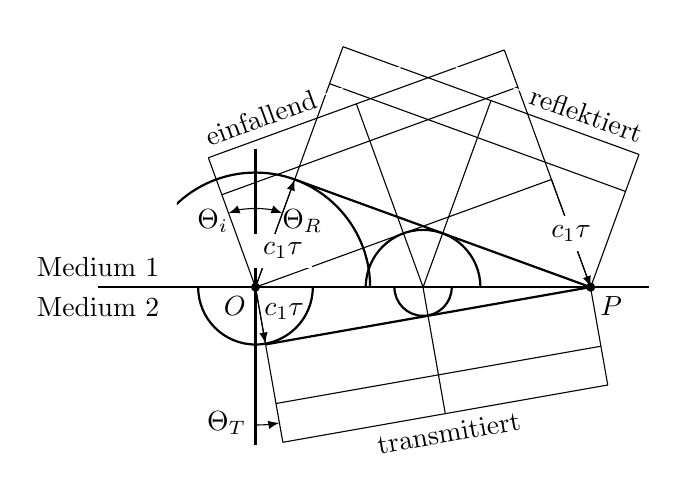
\begin{tikzpicture}[>=latex]
	\begin{scope}
		\clip (-1.5,0) rectangle (5,3.1);
		\foreach \i in {-1,1} {
			\begin{scope}[rotate=\i*20,yshift=-2cm-\i*.75cm]
				\foreach \i in {0,1,2}
					\draw (\i*2,0) -- (\i*2,4.5);
				\foreach \i in {0,1}
					\draw (0,\i*.5+4) -- (4,\i*.5+4);
			\end{scope}
		}
	\end{scope}
	
	\begin{scope}
		\clip (-.01,0) rectangle (5,-2);
		\begin{scope}[rotate=190,yshift=-2.5cm,xshift=-4.19cm,xscale=1.0475]
			\foreach \i in {0,1,2}
				\draw (\i*2,0) -- (\i*2,4.5);
			\foreach \i in {0,1}
				\draw (0,\i*.5+4) -- (4,\i*.5+4);
		\end{scope}
	\end{scope}
	
	\begin{scope}
		\draw[thick] (-2,0) node[above]{Medium 1} node[below]{Medium 2} -- (5,0)
		(0,-2) -- (0,1.75);
		
		\draw[thick,rotate=-20,yshift=1.45588cm] (4,0) -- (0,0);
		\draw[rotate=20,yshift=0cm] (4,0) -- (0,0);
		\draw[thick,rotate=190,yshift=1.45588cm/2+.1mm,xscale=1.0475] (-4,0) -- (0,0);
		
	\end{scope}
	
	\begin{scope}
		\clip (-1,0) rectangle (4,1.5);
		\draw[thick] (0,0) circle (1.45588cm);
		\draw[thick] (2.1284,0) circle (1.45588cm/2);
	\end{scope}

	\begin{scope}
		\clip (-1,0) rectangle (4,-1.5);
		\draw[thick] (0,0) circle (1.45588cm/2);
		\draw[thick] (2.1284,0) circle (1.45588cm/4);
	\end{scope}
	
	\begin{scope}
		\draw[fill=black] (0,0) circle (.5mm) node[below left]{$O$};
		\draw[fill=black] (4.2567,0) circle (.5mm) node[below right]{$P$};
	\end{scope}
	
	\draw[rotate=20,yshift=2cm,color=white] (0,0) -- (4,0) node[pos=.2,rotate=20,color=black]{einfallend};
	\draw[rotate=-20,yshift=3.5cm,color=white] (0,0) -- (4,0) node[pos=.8,rotate=-20,color=black]{reflektiert};
	\draw[rotate=10,yshift=-2.25cm,color=white,xscale=1.0475] (0,0) -- (4,0) node[pos=.5,rotate=10,color=black]{transmitiert};
	
	\draw[->] (0,1) arc (90:110:1cm) node[xshift=-2mm,yshift=-1mm]{$\Theta_i$};
	\draw[->] (0,1) arc (90:70:1cm) node[xshift=2.5mm,yshift=-1mm]{$\Theta_R$};
	\draw[->] (0,-1.75) arc (270:280:1.75cm) node[left,xshift=-3mm]{$\Theta_T$};
	
	\draw[->,rotate=-20] (0,0) -- (0,1.45588cm) node[pos=.3,fill=white,xshift=2mm,yshift=.5mm]{$c_1 \tau$};
	\draw[<-,rotate=20,yshift=-1.45588cm] (4,0) -- (4,1.45588cm) node[pos=.5,fill=white]{$c_1 \tau$};
	\draw[->,rotate=10] (0,0) -- (0,-1.45588cm/2) node[pos=.5,xshift=3mm,yshift=.5mm]{$c_1 \tau$};
	
\end{tikzpicture}
